	\documentclass[12pt,a4paper]{article}
\usepackage[utf8]{inputenc}
\usepackage{amsmath}
\usepackage{amsfonts}
\usepackage{amssymb}
\usepackage{listings}
\usepackage{url}
\usepackage[bulgarian]{babel}
\usepackage{listings}
\usepackage{enumerate}
\usepackage{hyperref}
\usepackage{relsize}
\usepackage{graphicx}
\usepackage{hyperref}
\usepackage{mathtools}


\lstset{breaklines=true}


\author{\textit{email: kalin@fmi.uni-sofia.bg}}
\title{\textsc{Задачи за задължителна самоподготовка} \\
по \\
Структури от данни и програмиране\\
\textit{Двоични дървета 3}}



\begin{document}
\maketitle


\begin{enumerate}

	\item Дадено е двоично дърво. Да се напише функция, проверяваща дали има поне две различни нива от дървото, чиито множества от елементи съвпадат.

	\item Да се реализира метод \texttt{bool BTree<T>::isBOT()},който проверява дали двоичното дърво е наредено.


	\begin{flushleft}
	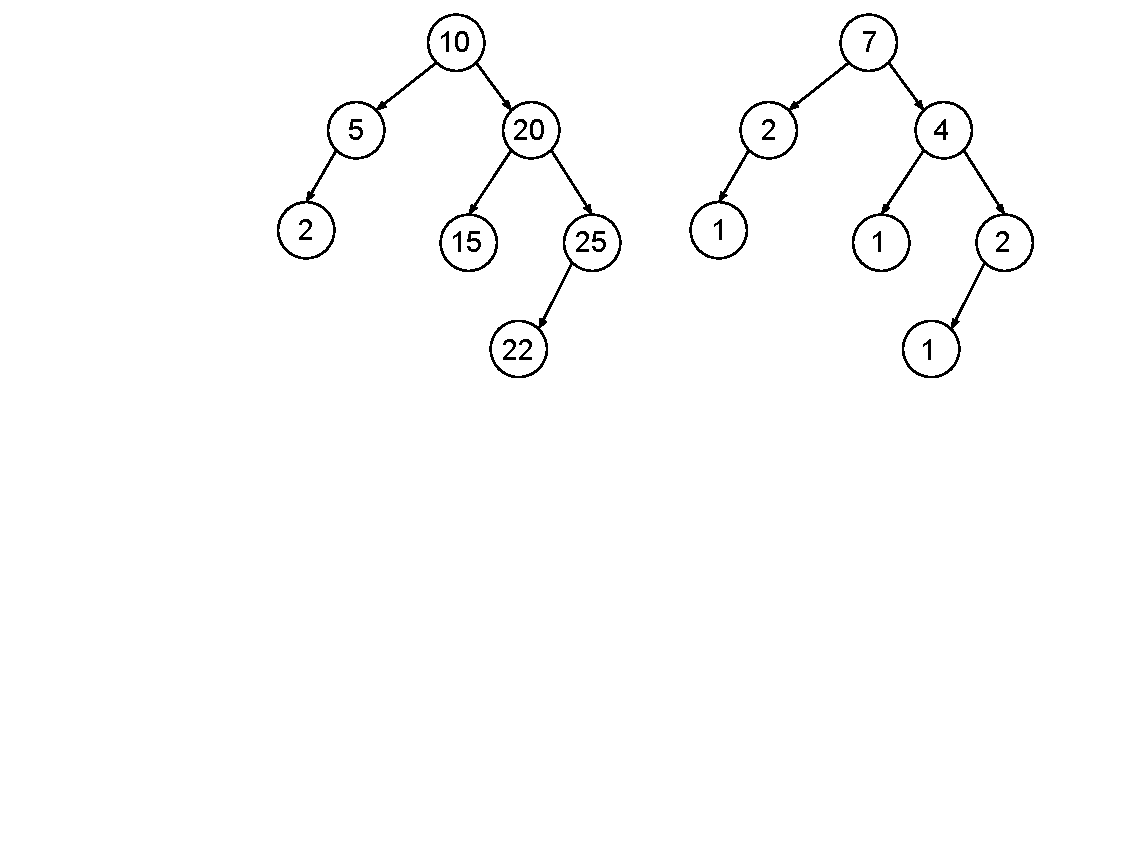
\includegraphics[width=9cm]{images/tree1}

	\vspace{-100px}

	\relscale{0.8}
	Фигура 1. Примерно дърво и същото дърво, стойностите на чиито възли са заместени с размера на съответното им поддърво.
	\end{flushleft}

	\item Стойността на всеки възел \texttt{V} в дадено двоично дърво от числа да се замени с броя на всички елементи на поддървото, на което \texttt{V} е корен. Вж. фигура 1. При операцията всеки от възлите да бъде посетен най-много веднъж.

	\item Нека е дадена матрица от цели числа $A_{M\times N}$ с елементи $(a_{i,j})$. ``Лява'' подматрица на $A$ наричаме такава подматрица $A'_{M'\times N'}$ на $A$, всеки елемент на която е по-малък от $a_{0,0}$. ``Дясна'' подматрица на $A$ наричаме такава подматрица $A'_{M'\times N'}$ на $A$, всеки елемент на която е по-голям от $a_{0,0}$.


	\begin{flushleft}
	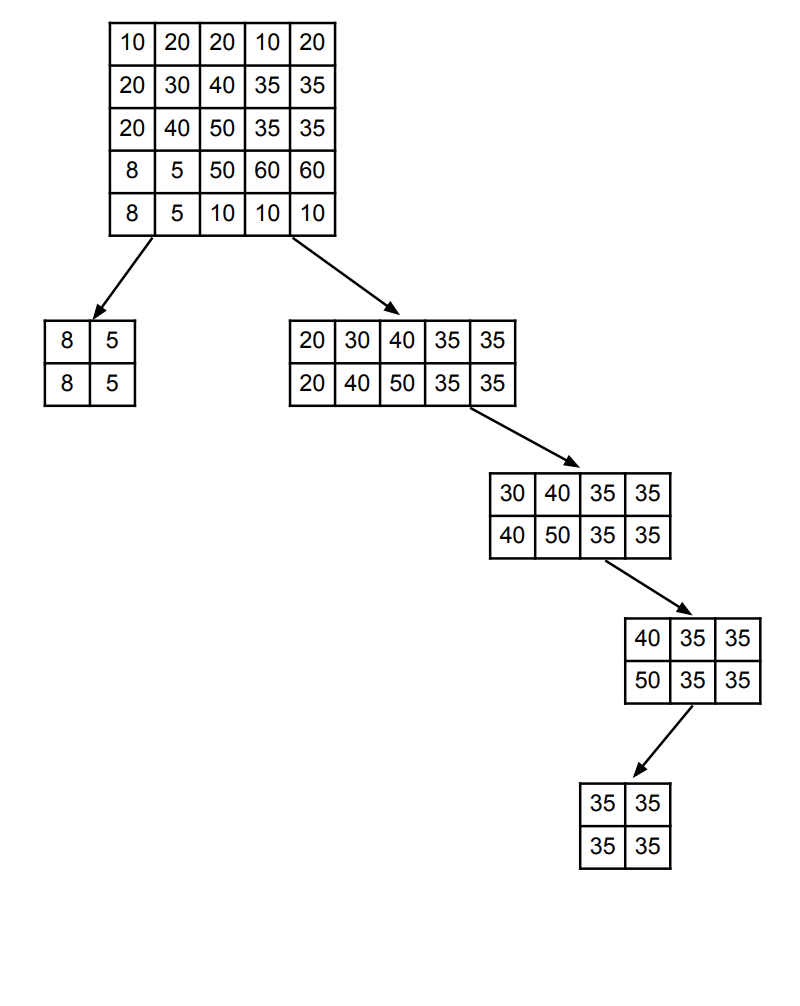
\includegraphics[width=9cm]{images/tree3}

	\relscale{0.8}
	Фигура 2. Наредено дърво от матрици.
	\end{flushleft}

	По матрицата $A$ да се построи двоично дърво $T$ със следните свойства:

	\begin{itemize}
		\item Коренът на $T$ съдържа матрицата $A$.
		\item Нека $v$ е произволен възел от дървото $T$, съдържащ матрица $X$. Ако $X$ има поне една лява подматрица с размер поне $2 \times 2$, то левият наследник на $X$ съдържа най-голямата (по брой елементи) лява подматрица на $X$. Ако има повече от една лявва подматрциа с максимален брой елементи, то левият наследник на $v$ е произволна една от тях. Ако $X$ няма лява подматрица с размер поне $2 \times 2$, то $v$ няма ляв наследник.
		\item Аналлогичното свойство за десния наследник на $v$ и най-голямата дясна подматрица (подматрици) на $X$.
	\end{itemize}

	На фигура 2 е изобразено едно такова дърво.

	\begin{enumerate}
		\item Да се избере подходящо представяне на матрици и на двоично дърво с матрици по върховете.
		\item Да се дефинира функция за построяване на дърво по горното правило по дадена матрица за корена му.
		\item Да се отпечата дървото чрез Graphviz. Повече информация за отпечатване на матрици като елемент на дървото може да се намери в \href{http://www.graphviz.org/content/node-shapes}{документацията на Graphviz}.
	\end{enumerate}


	\item Дадено е дърво с низове по върховете. Дървото да се балансира по следния начин:

	\begin{flushleft}
	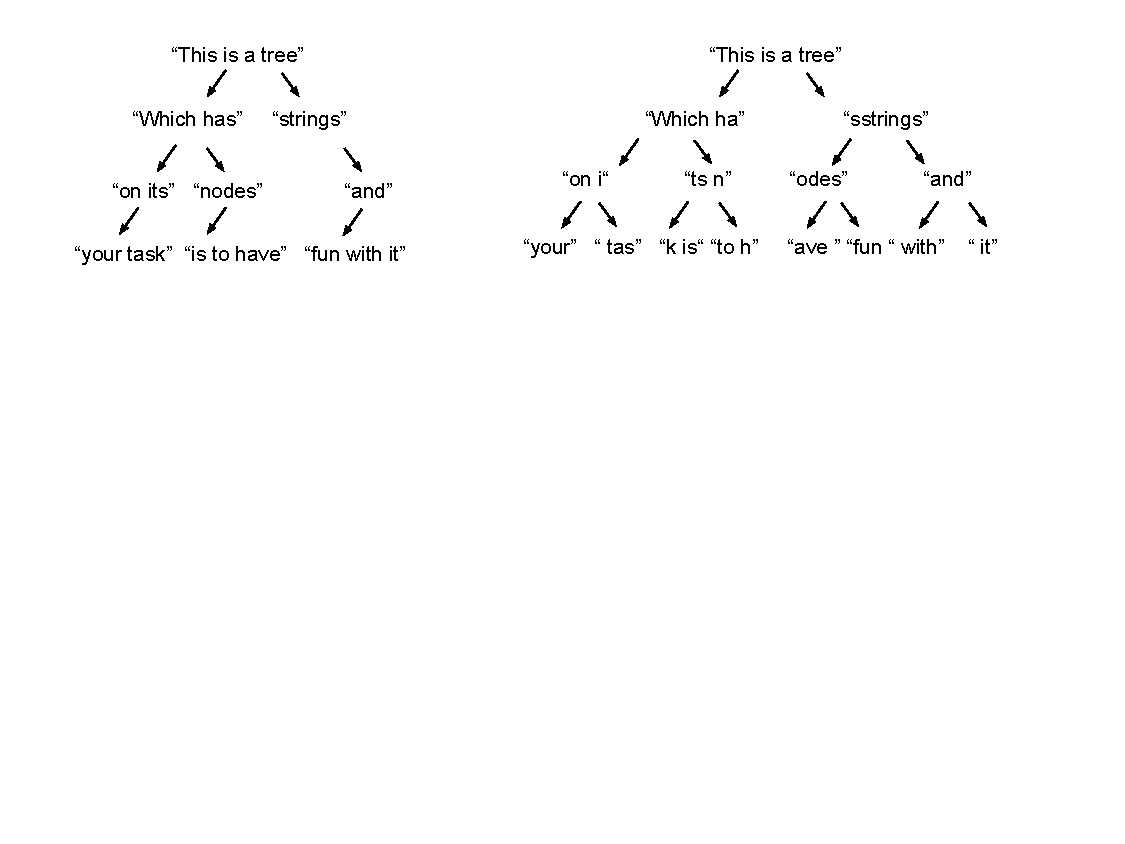
\includegraphics[width=15cm]{images/tree4}

	\vspace{-200px}

	\relscale{0.8}
	Фигура 3. Примерно дърво от низове преди и след балансирането.
	\end{flushleft}


	\begin{enumerate}
	  \item Резултатното дърво има същия брой нива като изходното.
		\item Всяко $k$-то ниво на резултатното дърво да съдържа точно $2^k$ елемента (считаме, че коренът е на ниво 0).
		\item Нека $s_k$ е низът, получен при конкатенацията на всички низове на ниво $k$ на изходното дърво, обхождани от ляво надясно. Нека дължината на низа е $n_k$ символа. $i$-тият пореден елемент на нивото $k$ в резултатното дърво да съдържа $i$-тата поредна последнователност от $\lceil{n_k/{2^k}}\rceil$ на брой символи на $s_k$, освен най-десния, който съдържа последните ``останали'' символи от $s_k$.
	\end{enumerate}

	На фигура 3 са илюстрирани примерно изходно дърво и резултатът от балансирането му по горното правило. Всички елементи на ниво 1, освен последния, съдържат по $8=\lceil{16/2}\rceil$ символа. Всички елементи на ниво 2, освен последния, съдържат по $4=\lceil{14/4}\rceil$ символа и т.н.


	\emph{Упътване: предварително намерете вектора $(s_0,s_1,...,s_{h-1})$ и го използвайте за балансирането.}

\end{enumerate}






\end{document}
